% !TEX root = Master.tex



This pair of clusters also let's us speculate whether tail dependence exists (see \autoref{fig:scatter_res_kcc_68}).
\\


\begin{figure}[H]
\centering
  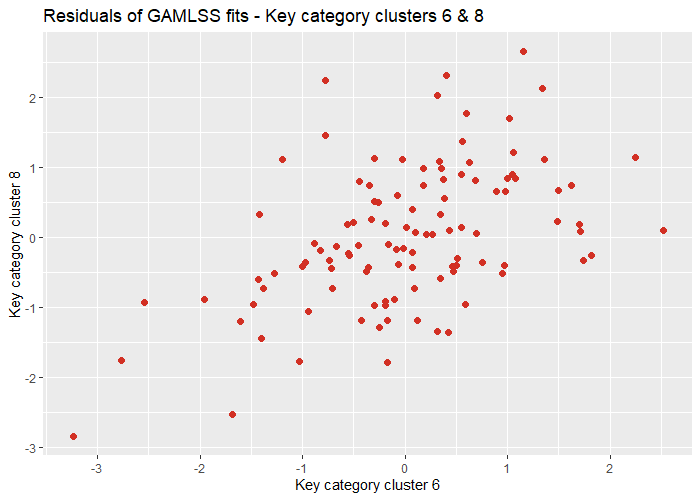
\includegraphics[width=0.45\linewidth]{figures/scatter_res_kcc_68.png}
  \caption{Scatterplot of estimated residuals of GAMLSS fits for key category clusters 6 \& 8}
  \label{fig:scatter_res_kcc_68}
\end{figure}


This time we fast forward to the outcome when a t-copula is applied (which is the proposed family of copulas allowing both concordance directions) under similar conditions as in Model \ref{eq:gjrm_formula_28} (the reasons for leaving out promo type being the same as in Subsection \ref{sssec:kcc_28}). Interestingly, the correlation parameter seems to be purely non-negative\footnote{Without considering the lower confidence bounds in the first part of the time window.} (see \autoref{fig:estimated_theta_t_copula_kcc_68}).
\\


\begin{figure}[H]
\centering
  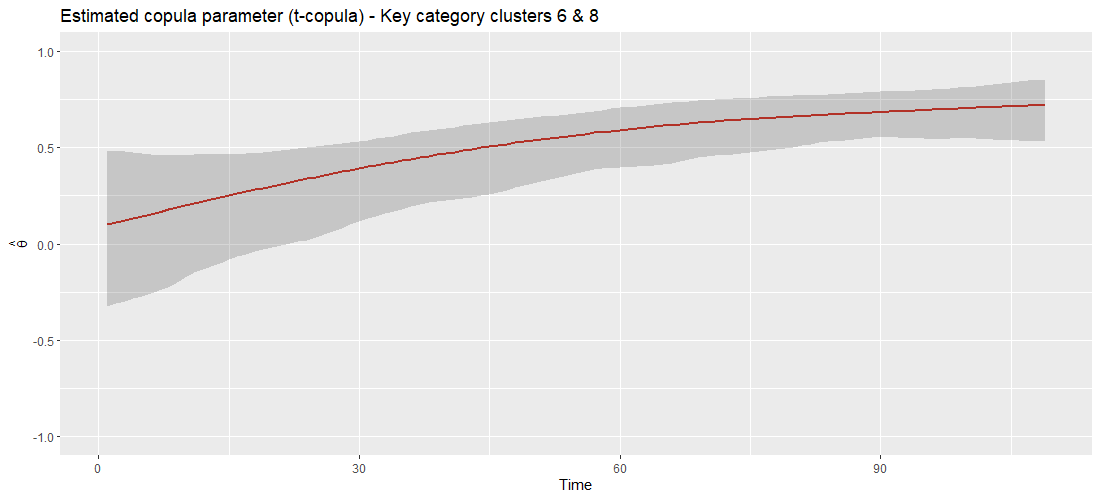
\includegraphics[width=0.95\linewidth]{figures/estimated_theta_t_copula_kcc_68.png}
  \caption{Estimated copula parameter over time from a \ac{GJRM} t-copula model with normal margins for key category clusters 6 \& 8 with 95\% confidence bands}
  \label{fig:estimated_theta_t_copula_kcc_68}
\end{figure}


Keeping the complexity of the model to a minimum, the model setup remains as is, with the only minor differences. Other copula families are considered in addition, particularly those that account for positive (and not negative) dependencies. Out of all implemented copula families in the \textit{VineCopula} package (rotated versions included), the Clayton copula yields the most fitting family for the given target variables. This result is sensible, as the Clayton copula is able to capture lower tail dependencies (\autoref{fig:scatter_res_kcc_68}) and accounts for positive dependence structures only (see Subsections \ref{sssec:archimedean_copulas} and \ref{sssec:tail_dependence}). Note that the new model specification is \\

\begin{equation}
\begin{array}{c}
\mu_{KCC 6}=\beta_{\mu,KCC6} \qquad \mu_{KCC 8}=\beta_{\mu,KCC8}  \\  \noalign{\vskip5pt}

log(\sigma_{KCC 6})=\beta_{\sigma,KCC6} \qquad log(\sigma_{KCC 8})=\beta_{\sigma,KCC8} \\  \noalign{\vskip5pt}


log(\theta)=\beta_{\theta}+f\left(t_{time}\right),
\end{array}
\label{eq:gjrm_formula_68}
\end{equation}
\\

where now there are no degrees of freedom to determine and the copula parameter receives a logarithmic link function to ensure that $\hat{\theta}$ is well defined on the non-negative real line. Equation 5 in R output \ref{output:summary_kcc_68} shows the significance of time on $\hat{\theta}$ and its smooth effect is visualized in \autoref{fig:time_effect_on_theta_68}. The diagnostic plots of quantile residuals in \autoref{fig:res_hist_qqplot_68} demonstrate the proper fit qualities once more.
\\


\inputRoutput[caption={Summary of GJRM fit on key category clusters 6 \& 8},numbers=left,numberstyle=\tiny, label=output:summary_kcc_68]{summary_kcc_68.txt}


\begin{figure}[H]
\centering
  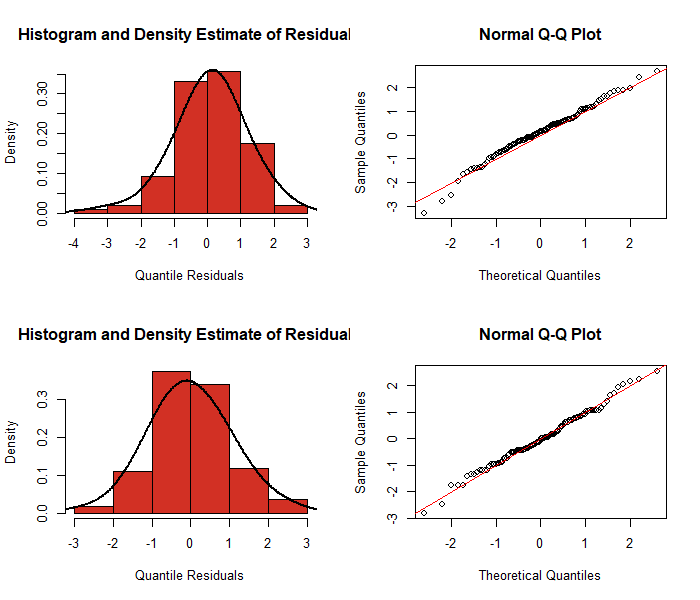
\includegraphics[width=0.95\linewidth]{figures/res_hist_qqplot_68.png}
  \caption{Diagnostic plots of quantile residuals based on \ac{GJRM} models for key category clusters 6 \& 8}
  \label{fig:res_hist_qqplot_68}
\end{figure}




\begin{figure}[H]
\centering
  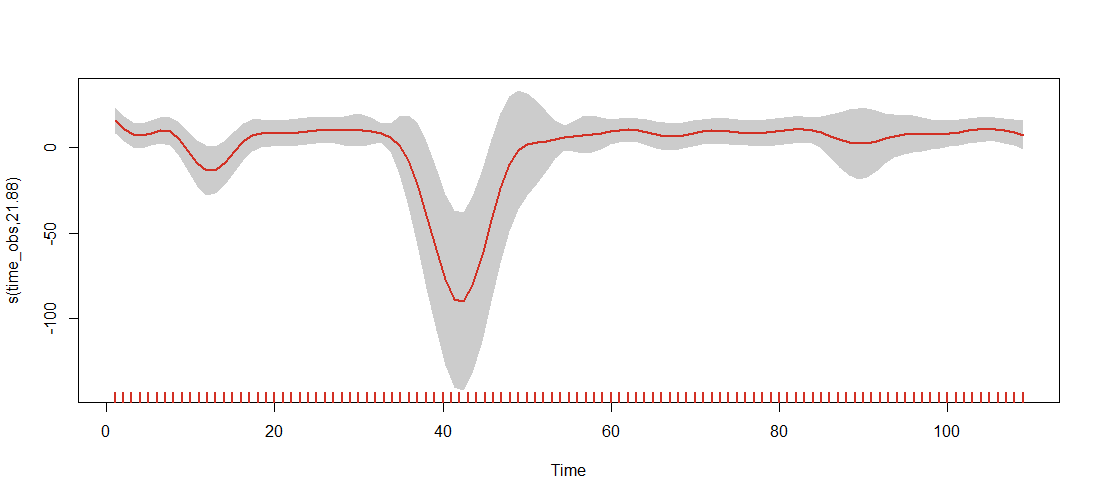
\includegraphics[width=0.95\linewidth]{figures/time_effect_on_theta_68.png}
  \caption{Estimated Smooth effect of time on the copula parameter $\theta$ with 95\% confidence bands for key category clusters 6 \& 8}
  \label{fig:time_effect_on_theta_68}
\end{figure}



Since Kendall's tau is more intuitive as a dependence measure of two random variables than the copula parameter $\theta$ (see Subsection \ref{sssec:rank_correlation}), this is what we inspect. The relationship between Kendall's tau and the parameter of the Clayton copula is $\tau = \frac{\theta}{\theta + 2}$ (see \autoref{tab:copula_relationships}). The estimated time-varying $\hat{\tau}$ is displayed in \autoref{fig:estimated_tau_clayton_kcc_68}, where we can observe that 
%the confidence bands vary a lot and 
there are some individual time windows of zero correlation.\\

Any model configuration of this pair regarding covariates and copulas produce such kind of strictly non-negative dependence. These results should be interpreted with extraordinary caution if at all.
\\



\begin{figure}[H]
\centering
  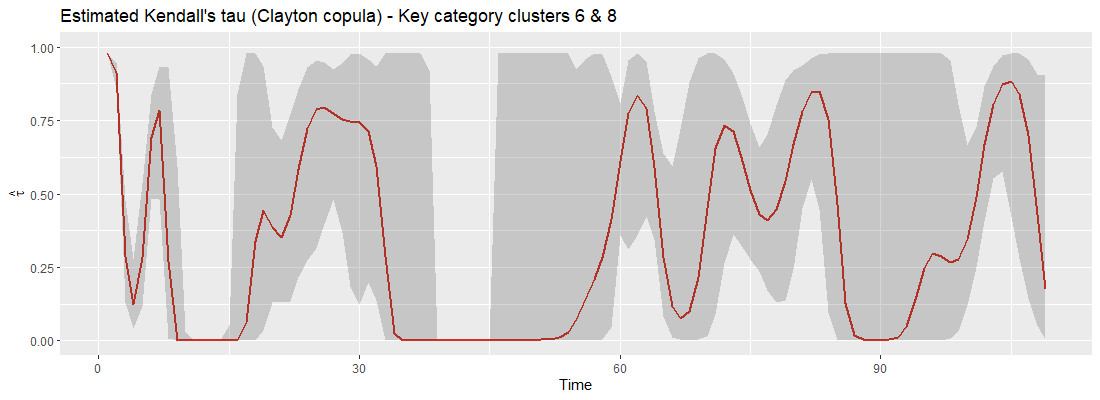
\includegraphics[width=0.95\linewidth]{figures/estimated_tau_clayton_kcc_68.png}
  \caption{Estimated Kendall's tau over time and 95\% confidence bands from a \ac{GJRM} Clayton copula model with normal margins for key category clusters 6 \& 8 - Season type in the background - Dashed horizontal line at $\hat{\theta} = 0$}
  \label{fig:estimated_tau_clayton_kcc_68}
\end{figure}
% - Confidence bands are neglected for clarity of the graph

































%The \ac{GJRM} fit on this pair seems to work just fine, which is underlined when observing \autoref{fig:margin_estimates_kcc_68}. As for the estimation of the dependence, we obtain a similar scheme as in the pair \ac{KCC} 2 \& \ac{KCC} 8. The main course of the correlation coefficient is common for both approaches, however the gamCopula approach seems to reveal heavier fluctuations. As always, it shall be stressed that these conclusions should be taken into account with extra caution, as both algorithms converge.
%
%\begin{figure}[H]
%\centering
%  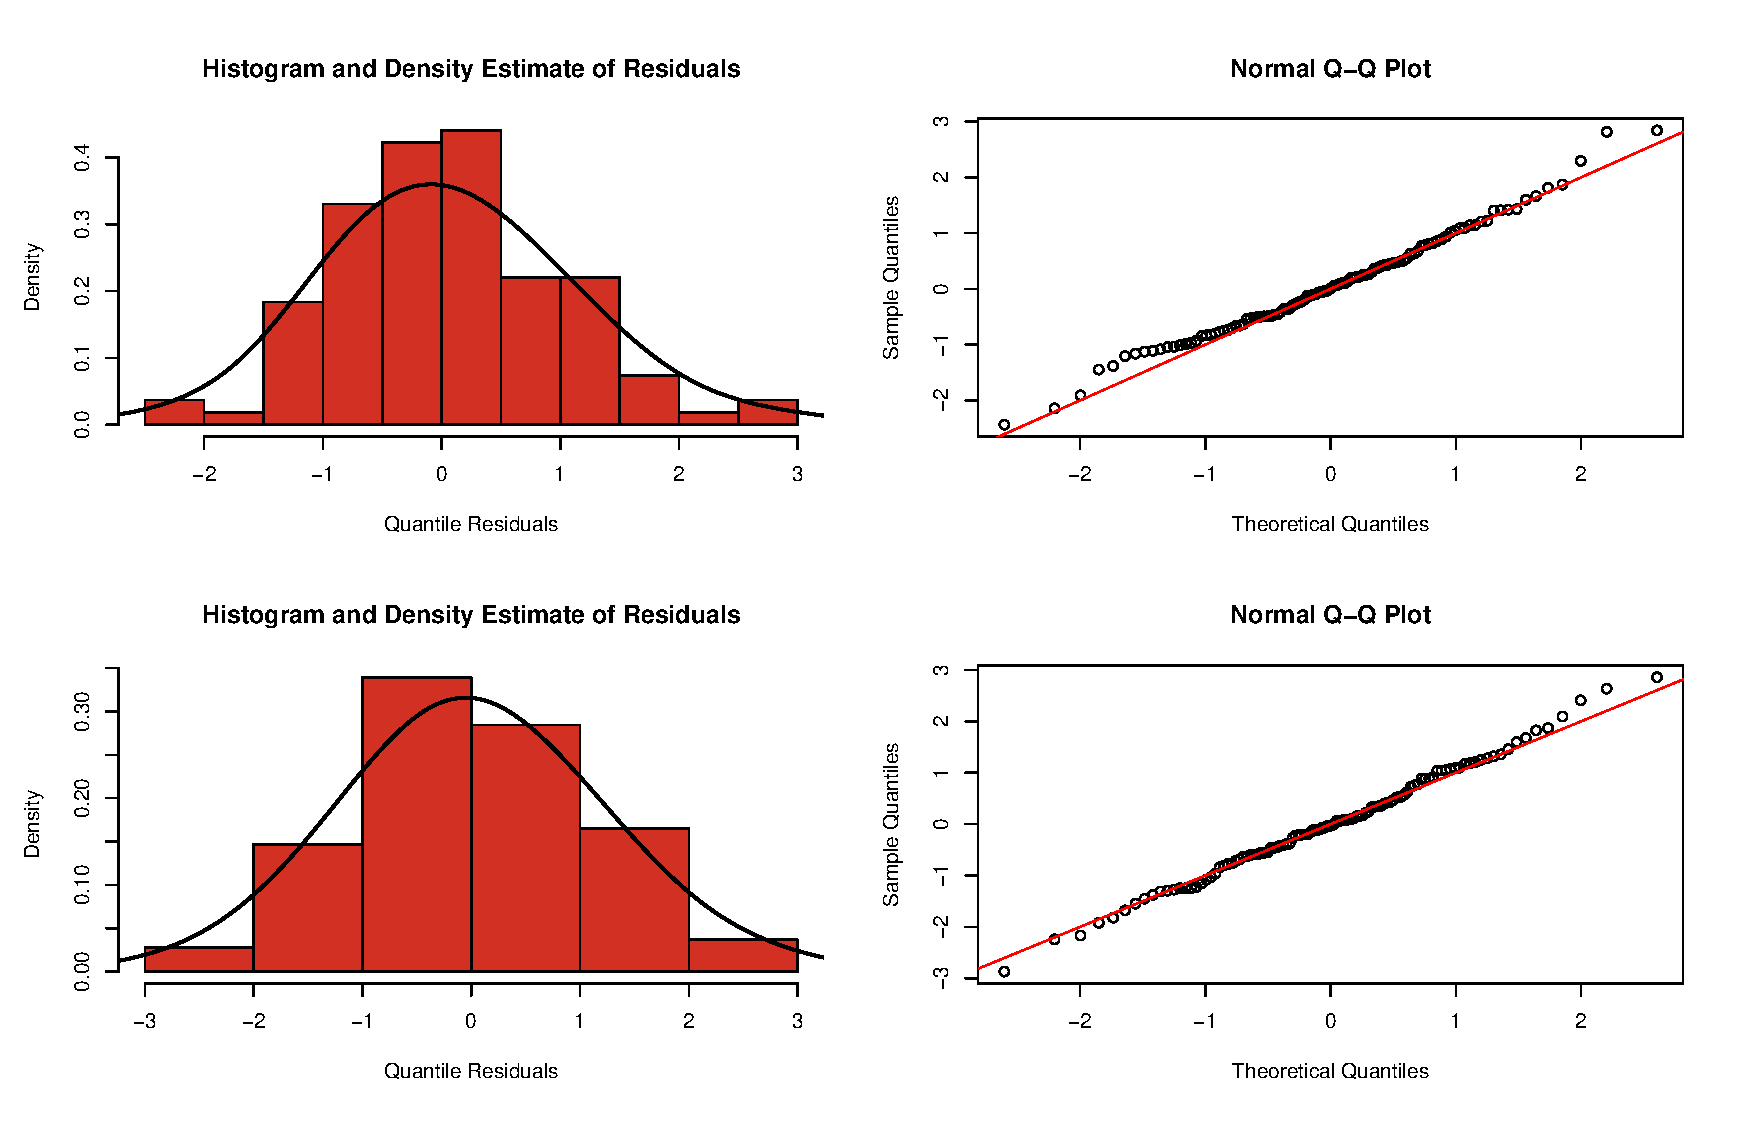
\includegraphics[width=0.9\linewidth]{figures/margin_estimates_kcc_68.eps}
%  \caption{Estimation diagnostics for the response margins KCC 6 \& KCC 8; \ac{GJRM} approach}
%  \label{fig:margin_estimates_kcc_68}
%\end{figure}
% 
%
%
%
%\begin{figure}[H]
%\centering
%  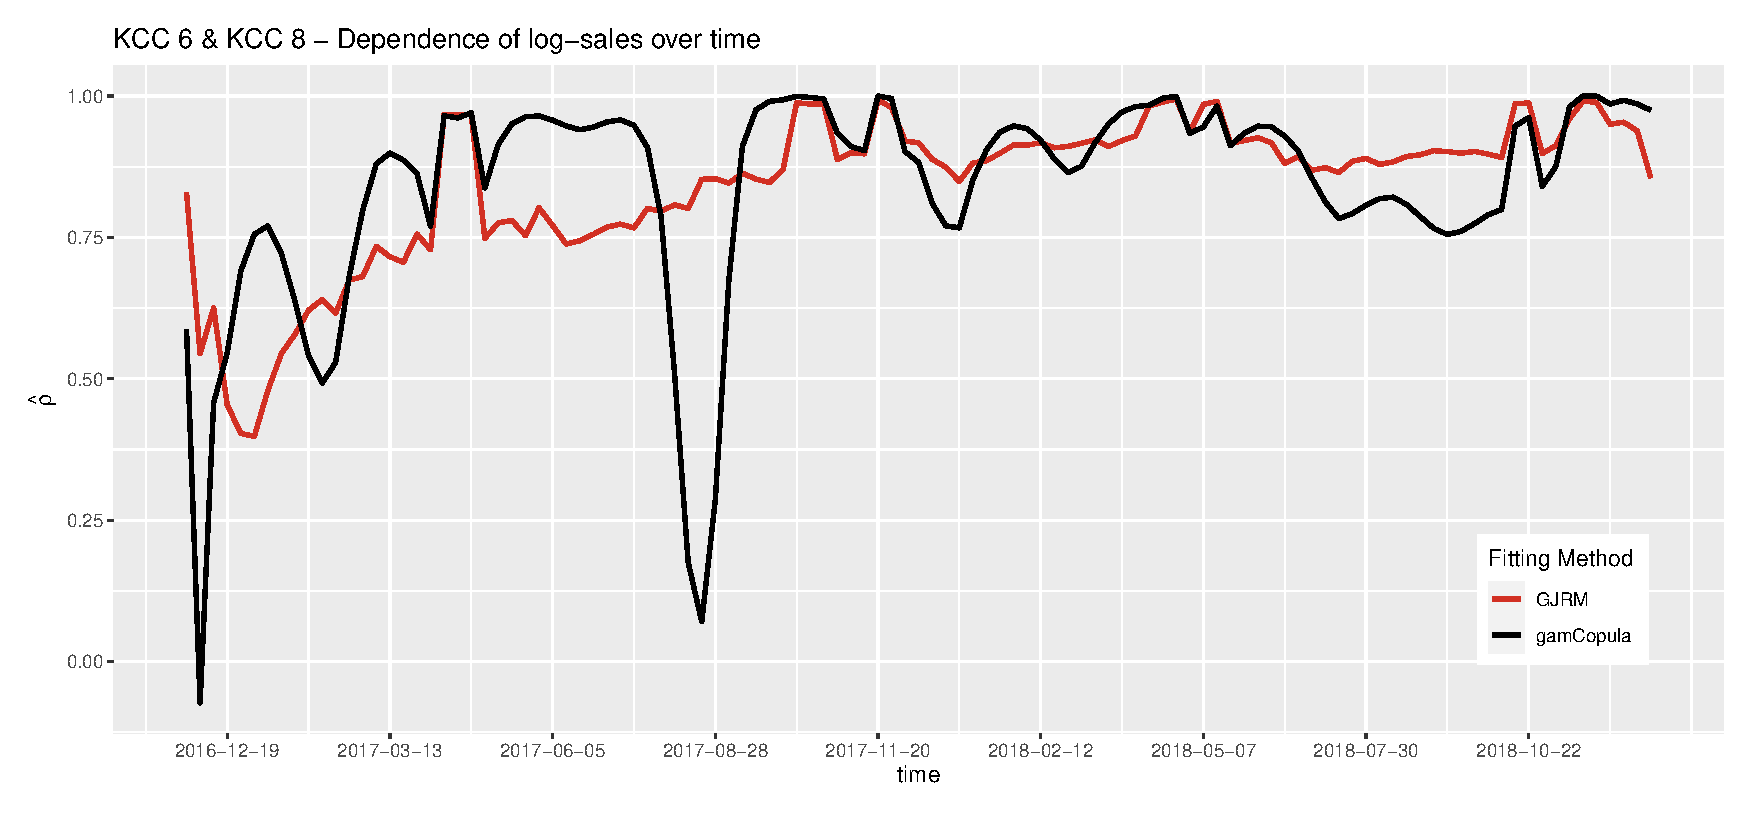
\includegraphics[width=0.9\linewidth]{figures/copula_parameters_68.eps}
%  \caption{Estimated time-varying Pearson's correlation coefficients for the pair KCC 6 \& KCC 8}
%  \label{fig:copula_parameters_68}
%\end{figure}
%
%
%
%In both correlations in \autoref{fig:copula_parameters_68} show an overall increasing trend from the start, which stabilizes somewhere in September of 2017. Both curves return positive values throughout the entire time span (except for the very start of the black one). Also, wider and heavier fluctuations occur in the gamCopula approach as opposed to the \ac{GJRM} method, which looks much smoother.